%%%%%%%%%%%%%%%%%%%%%%%%%%%%%%%%%%%%%%%%%%%%%%%%%%%%%%%%%%%%%%%%%%%%%%
\begin{frame}[fragile]\frametitle{}
\begin{center}
{\Large Patterns and Tricks}
\end{center}
\end{frame}

%%%%%%%%%%%%%%%%%%%%%%%%%%%%%%%%%%%%%%%%%%%%%%%%%%%%%%%%%%%%%%%%%%%%%%
\begin{frame}[fragile]
	\frametitle{Two Pointers}
	
	\begin{columns}[T]
		\column{0.5\linewidth}	
			\begin{itemize}
				\item Two pointers iterate through the data structure in tandem until one or both of the pointers hit a certain condition.
				\item Two Pointers is often useful when searching pairs in a sorted array or linked list; 
				\item Two pointers are needed because with just pointer, you would have to continually loop back through the array to find the answer. 
				\item Examples:
			\begin{itemize}
				\item Squaring a sorted array (easy)
				\item Triplets that sum to zero (medium)
				\item Comparing strings that contain backspaces (medium)
			\end{itemize}

			\end{itemize}
			
		\column{0.5\linewidth}
		
\begin{center}
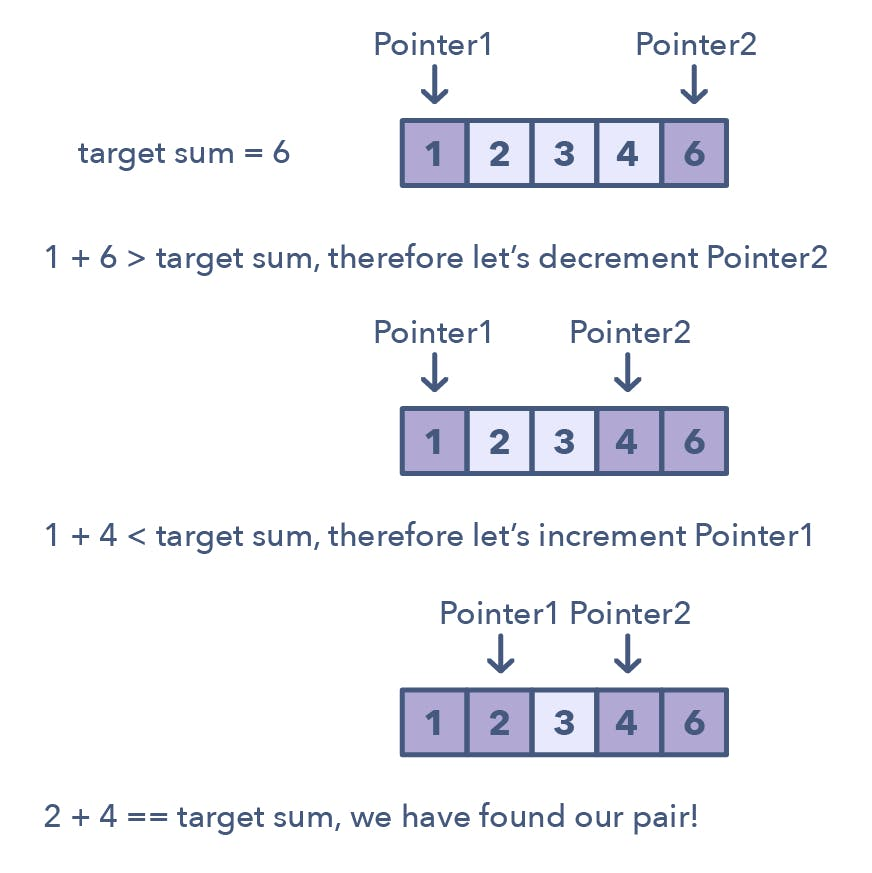
\includegraphics[width=\linewidth,keepaspectratio]{dsa2}
\end{center}			
	\end{columns}
\end{frame}

%%%%%%%%%%%%%%%%%%%%%%%%%%%%%%%%%%%%%%%%%%%%%%%%%%%%%%%%%%%%%%%%%%%%%%
\begin{frame}[fragile]
	\frametitle{Two Pointers}
	
We move from the left and right with different conditions until there’s something we want to find.

		
\begin{lstlisting}
/* General two pointer problem solution */ 
public boolean twoSumProblem(int A[], int N, int X)  
{  
    int left = 0;  // represents first pointer  
    int right = N - 1;  // represents second pointer  
    while (left < right) {  
        if(){ // question condition match 
            // do something 
            return true 
        } 
        else if(){ // first wrong condition 
            left+=1; // close in the array from left 
        } 
        else{ // second wrong condition 
            right-=1; // close in the array from right 
        } 
    }  
    return false;  
}  				
\end{lstlisting}			
\end{frame}


%%%%%%%%%%%%%%%%%%%%%%%%%%%%%%%%%%%%%%%%%%%%%%%%%%%%%%%%%%%%%%%%%%%%%%
\begin{frame}[fragile]
	\frametitle{Remove duplicates}
	
	\begin{columns}[T]
		\column{0.5\linewidth}	
			\begin{itemize}
				\item  One brute force way is to have a separate array, iterate over the original array and 
then add the items other than value to the new array.
				\item If the number is not ‘value’, bring to front, finally return the pointer. 
\item Shift the elements behind if they don’t match the value given.  
\item If we don’t have a value and just want to remove the duplicates and return the index.: Sill have 2 pointers, test if \lstinline|slow != fast| $\rightarrow$ move the slow pointer forward, and change the 
\lstinline|nums[slow]| to the fast one $\rightarrow$ basically pushing that element back. 
			\end{itemize}
			
		\column{0.5\linewidth}
		
\begin{lstlisting}
int removeElement(int A[], int elem) { 
    int pointer = 0; 
    for(int i=0; i<n; i++) { 
      if(A[i]!=elem) { 
        A[pointer++] = A[i]; 
      } 
    } 
    return pointer; 
}  	

def removeDuplicates(self, nums: List[int]) -> int: 
    if len(nums) ==0 : return 0 
    slow = 0 
    for fast in range(1,len(nums)): 
        if nums[slow] != nums[fast]: 
            slow += 1 
            nums[slow] = nums[fast] 
    return tail+1 			
\end{lstlisting}			
	\end{columns}
\end{frame}


%%%%%%%%%%%%%%%%%%%%%%%%%%%%%%%%%%%%%%%%%%%%%%%%%%%%%%%%%%%%%%%%%%%%%%
\begin{frame}[fragile]
	\frametitle{Two Sum $+$ Sorted}
	
	\begin{columns}[T]
		\column{0.5\linewidth}	
			\begin{itemize}
				\item  If we want to find 2 indices which sum up to a target and the array is sorted, we can start from left 
and right with 2 pointers, and move them according to the sum at every time. 
				\item Eventually we will find the target from those 2 indices, or just return -1 if we don’t.  
				\item However, the logic would be more complex if the array is not sorted. 
				\item We can simply store the elements 
in a hashmap as we go, and eventually return when we find $target-nums[i]$ in the array as we’re going 
forward. 
			\end{itemize}
			
		\column{0.5\linewidth}
		
\begin{lstlisting}
boolean pairSum(int A[], int N, int X)  
{  
    int i = 0; 
    int j = N - 1;  
   
    while (i < j) {  
        if (A[i] + A[j] == X)  
            return true;  
   
        else if (A[i] + A[j] < X)  
            i++;  
        else 
            j--;  
    }  
    return false;  
}  
\end{lstlisting}			
	\end{columns}
\end{frame}

%%%%%%%%%%%%%%%%%%%%%%%%%%%%%%%%%%%%%%%%%%%%%%%%%%%%%%%%%%%%%%%%%%%%%%
\begin{frame}[fragile]
	\frametitle{Sliding Window}
	
	\begin{columns}[T]
		\column{0.5\linewidth}		
			\begin{itemize}
				\item Used to perform a required operation on a specific window size of a given array or linked list
				\item Sliding Windows start from the 1st element and keep shifting right by one element and can adjust the length of the window 
				\item Window size can remain constant or grow - shrink.
				\item The problem input is a linear data structure such as linked list, array
				\item You’re asked to find the longest/shortest substring
			\end{itemize}
			
		\column{0.5\linewidth}
		
\begin{center}
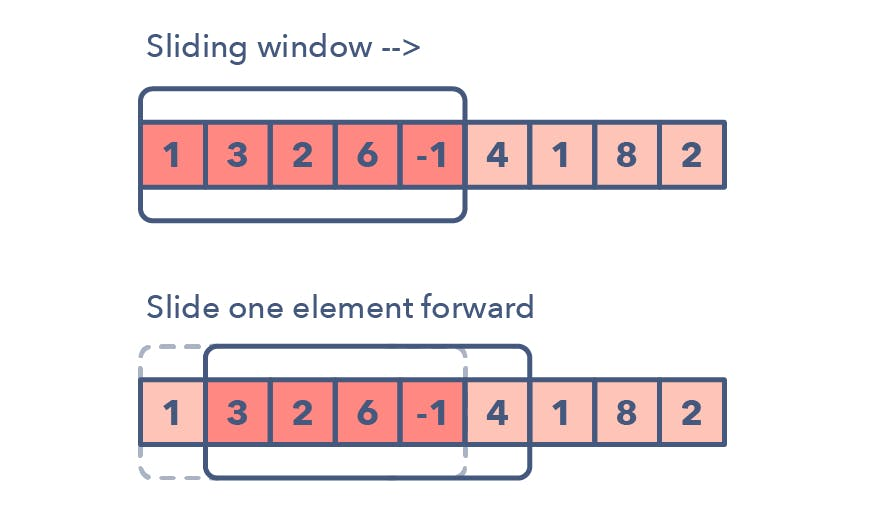
\includegraphics[width=\linewidth,keepaspectratio]{dsa1}
\end{center}	

Examples:
			\begin{itemize}
				\item Maximum sum subarray of size ‘K’ (easy)
				\item Longest substring with ‘K’ distinct characters (medium)
				\item String anagrams (hard)
			\end{itemize}
			
	\end{columns}		
\end{frame}

%%%%%%%%%%%%%%%%%%%%%%%%%%%%%%%%%%%%%%%%%%%%%%%%%%%%%%%%%%%%%%%%%%%%%%
\begin{frame}[fragile]
	\frametitle{Fast and Slow pointers}
	
	\begin{columns}[T]
		\column{0.5\linewidth}		
			\begin{itemize}
				\item Uses two pointers which move through the array (or sequence/linked list) at different speeds. 
				\item This approach is quite useful when dealing with cyclic linked lists or arrays.
				\item The fast pointer should catch the slow pointer once both the pointers are in a cyclic loop.
				\item Examples:
			\begin{itemize}
				\item Linked List Cycle (easy)
				\item Palindrome Linked List (medium)
				\item Cycle in a Circular Array (hard)
			\end{itemize}

			\end{itemize}
		\column{0.5\linewidth}
			
		
\begin{center}
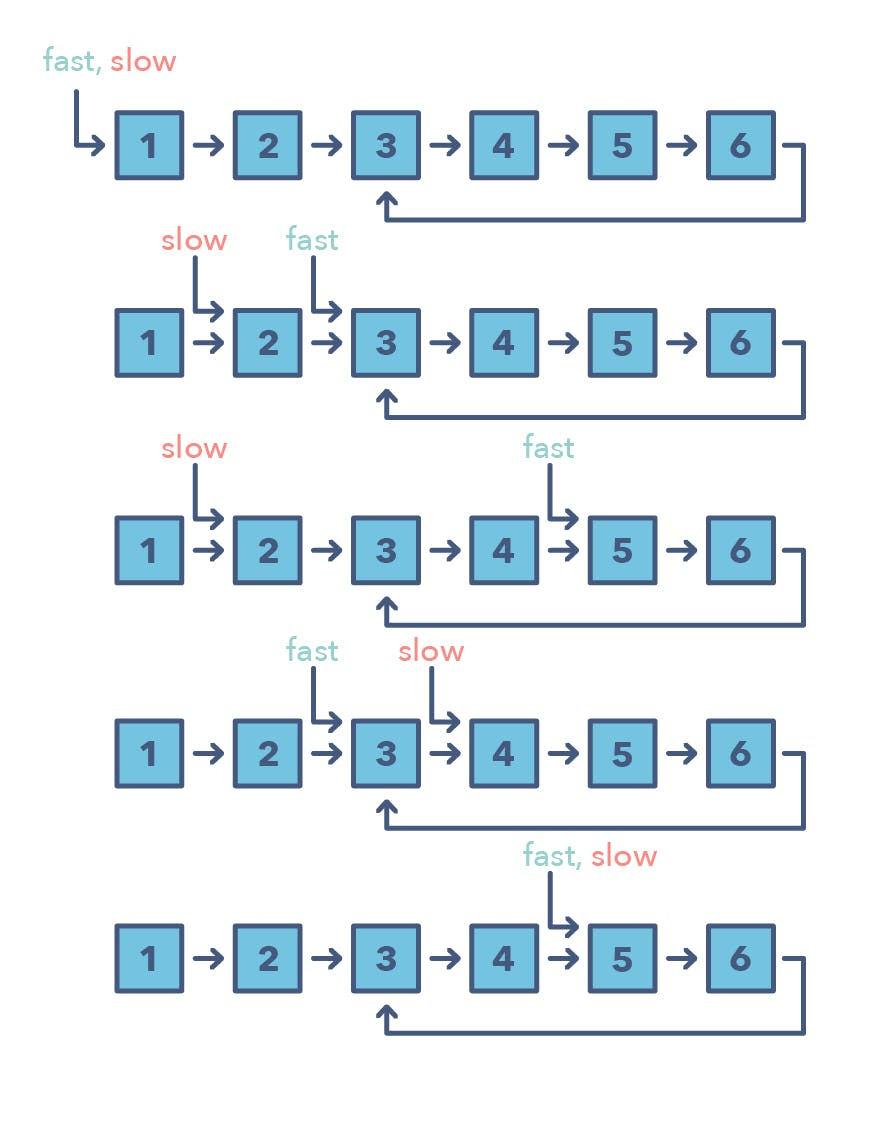
\includegraphics[width=\linewidth,keepaspectratio]{dsa3}
\end{center}			
	\end{columns}		
\end{frame}

%%%%%%%%%%%%%%%%%%%%%%%%%%%%%%%%%%%%%%%%%%%%%%%%%%%%%%%%%%%%%%%%%%%%%%
\begin{frame}[fragile]
	\frametitle{Linked List cycle}
	
	\begin{columns}[T]
		\column{0.5\linewidth}		
			\begin{itemize}
				\item  Idea: if we visit a node again, then we would find a cycle 
				\item  Store the nodes as you’re iterating and then see if you find the node in the set again.  But due to additional set, space complexity is there.
				\item Can we have a slow and fast pointer, where the fast tries to catch the slower one? If it can, we find a cycle.

			\end{itemize}
		\column{0.5\linewidth}
			
		
\begin{lstlisting}
public boolean hasCycle(ListNode head) { 
    Set<ListNode> set = new HashSet<>(); 
    while(head!=null){ 
        if(set.contains(head)){ 
            return true; 
        } 
        set.add(head); 
        head=head.next; 
    } 
    return false; 
} 			

while(runner.next!=null && runner.next.next!=null) { 
        walker = walker.next; 
        runner = runner.next.next; 
        if(walker==runner) return true; 
} 	
\end{lstlisting}			
	\end{columns}		
\end{frame}

%%%%%%%%%%%%%%%%%%%%%%%%%%%%%%%%%%%%%%%%%%%%%%%%%%%%%%%%%%%%%%%%%%%%%%
\begin{frame}[fragile]
	\frametitle{Merge Intervals}
	\begin{columns}[T]
		\column{0.5\linewidth}			
			\begin{itemize}
				\item In a lot of problems involving intervals, you either need to find overlapping intervals or merge intervals if they overlap. 
				\item The pattern works like this:

Given two intervals (‘a’ and ‘b’), there will be six different ways the two intervals can relate to each other (figure below):
				\item Examples:
			\begin{itemize}
				\item Intervals Intersection (medium)
				\item Maximum CPU Load (hard)
			\end{itemize}

			\end{itemize}
		\column{0.5\linewidth}
			
		
\begin{center}
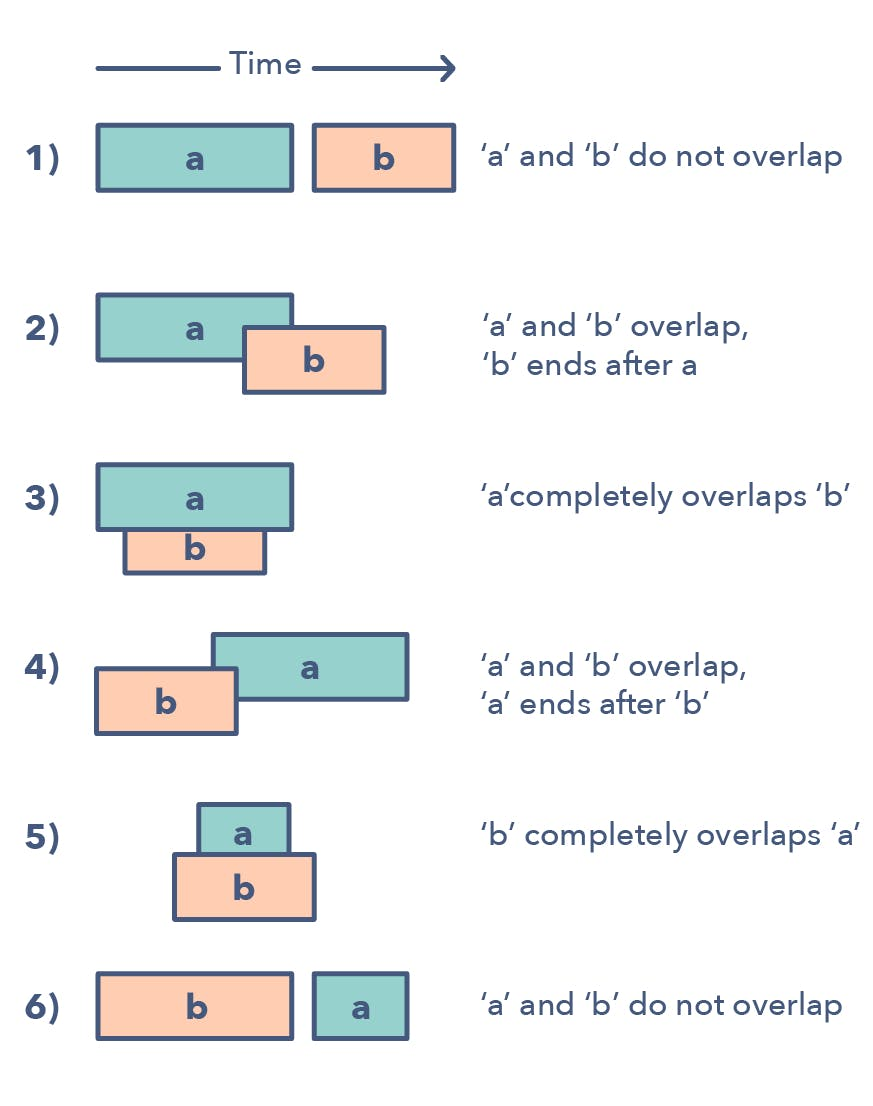
\includegraphics[width=\linewidth,keepaspectratio]{dsa4}
\end{center}		
		\end{columns}		
\end{frame}

%%%%%%%%%%%%%%%%%%%%%%%%%%%%%%%%%%%%%%%%%%%%%%%%%%%%%%%%%%%%%%%%%%%%%%
\begin{frame}[fragile]
	\frametitle{Cyclic sort}
	\begin{columns}[T]
		\column{0.5\linewidth}			
			\begin{itemize}
			\item To find the missing/duplicate/smallest number in an sorted/rotated array
				\item Iterates over the array one number at a time, and if the current number you are iterating is not at the correct index, you swap it with the number at its correct index. 
				\item You could try placing the number in its correct index, but this will produce a complexity of $O(n^2)$ which is not optimal, hence the Cyclic Sort pattern.
				\item Examples:
			\begin{itemize}
				\item Find the Missing Number (easy)
				\item Find the Smallest Missing Positive Number (medium)
			\end{itemize}

			\end{itemize}
		\column{0.5\linewidth}
			
		
\begin{center}
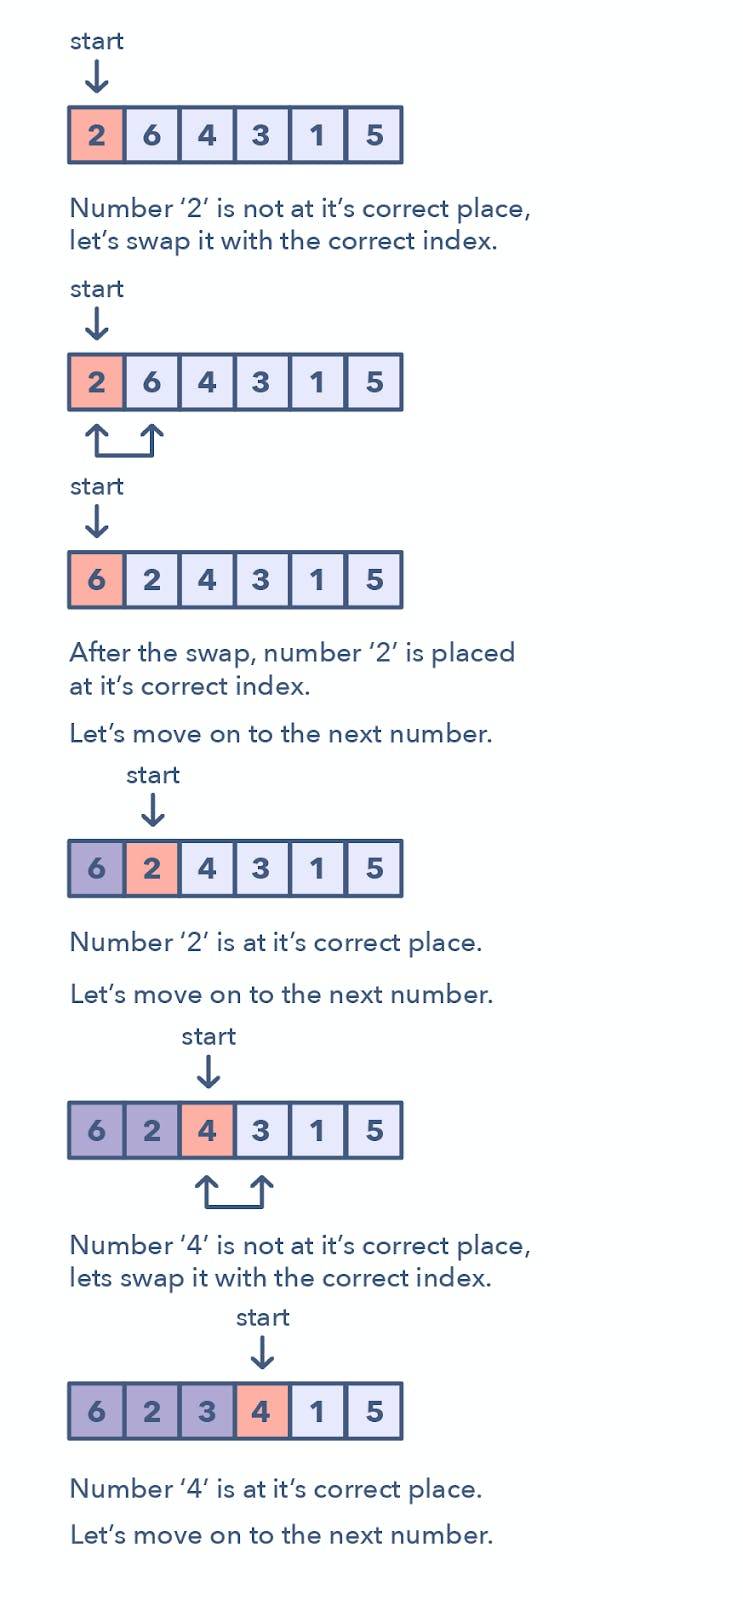
\includegraphics[width=0.8\linewidth,keepaspectratio]{dsa5}
\end{center}		
		\end{columns}		
\end{frame}

%%%%%%%%%%%%%%%%%%%%%%%%%%%%%%%%%%%%%%%%%%%%%%%%%%%%%%%%%%%%%%%%%%%%%%
\begin{frame}[fragile]
	\frametitle{In-place reversal of linked list}
	\begin{columns}[T]
		\column{0.5\linewidth}			
			\begin{itemize}
			\item Reverses one node at a time starting with one variable (current) pointing to the head of the linked list, and one variable (previous) will point to the previous node that you have processed. 
			\item In a lock-step manner, you will reverse the current node by pointing it to the previous before moving on to the next node. 
			\item Also, you will update the variable “previous” to always point to the previous node that you have processed.
				\item Examples:
			\begin{itemize}
				\item Reverse a Sub-list (medium)
				\item Reverse every K-element Sub-list (medium)
			\end{itemize}

			\end{itemize}
		\column{0.5\linewidth}
			
		
\begin{center}
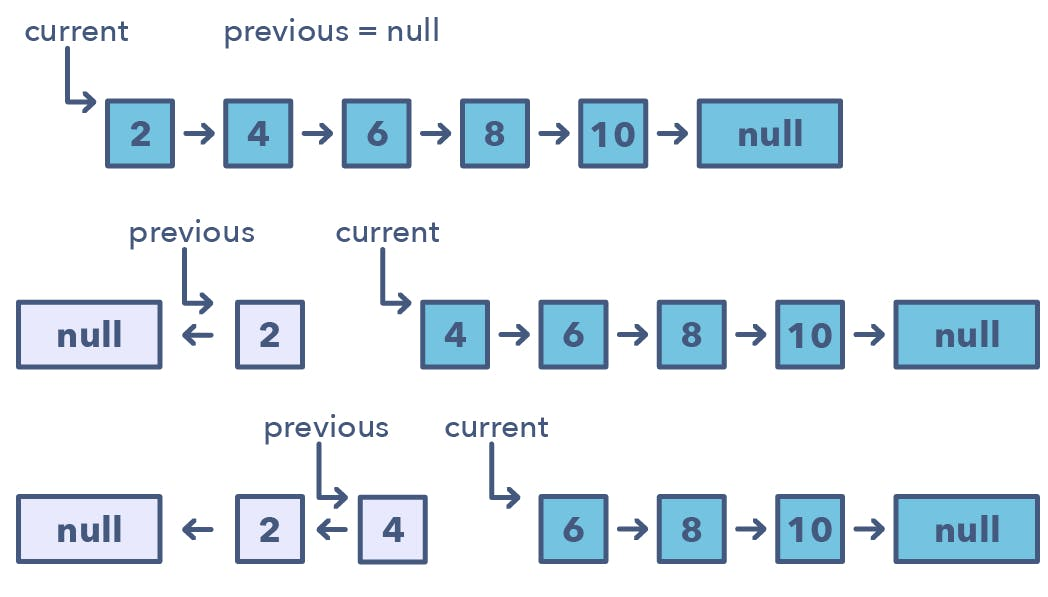
\includegraphics[width=\linewidth,keepaspectratio]{dsa6}
\end{center}		
		\end{columns}		
\end{frame}

%%%%%%%%%%%%%%%%%%%%%%%%%%%%%%%%%%%%%%%%%%%%%%%%%%%%%%%%%%%%%%%%%%%%%%
\begin{frame}[fragile]
	\frametitle{Tree Breadth First Search (BFS)}
		
			\begin{itemize}
			\item To traverse a tree and uses a queue to keep track of all the nodes of a level before jumping onto the next level.
			\item Works by pushing the root node to the queue and then continually iterating until the queue is empty. 
			\item For each iteration, we remove the node at the head of the queue and “visit” that node. 
			\item After removing each node from the queue, we also insert all of its children into the queue.
				\item Examples:
			\begin{itemize}
				\item Binary Tree Level Order Traversal (easy)
				\item Zigzag Traversal (medium)
			\end{itemize}

			\end{itemize}	
\end{frame}

%%%%%%%%%%%%%%%%%%%%%%%%%%%%%%%%%%%%%%%%%%%%%%%%%%%%%%%%%%%%%%%%%%%%%
\begin{frame}[fragile]
	\frametitle{Tree Depth First Search (DFS)}
		
			\begin{itemize}
			\item Use recursion (or a stack for the iterative approach) to keep track of all the previous (parent) nodes while traversing.
			\item Works by starting at the root of the tree, if the node is not a leaf you need to do three things:
			\begin{itemize}
			\item Decide whether to process the current node now (pre-order), or between processing two children (in-order) or after processing both children (post-order).
			\item Make two recursive calls for both the children of the current node to process them.
			\end{itemize}
			
				\item Examples:
			\begin{itemize}
				\item Sum of Path Numbers (medium)
				\item All Paths for a Sum (medium)
			\end{itemize}

			\end{itemize}	
\end{frame}

%%%%%%%%%%%%%%%%%%%%%%%%%%%%%%%%%%%%%%%%%%%%%%%%%%%%%%%%%%%%%%%%%%%%%%
\begin{frame}[fragile]
	\frametitle{Two heaps}
		
			\begin{itemize}
			\item Elements are divided in two parts
			\item Interested in knowing the smallest element in one part and the biggest element in the other part.
			\item Uses two heaps; A Min Heap to find the smallest element and a Max Heap to find the biggest element. 
			\item The pattern works by storing the first half of numbers in a Max Heap, this is because you want to find the largest number in the first half. You then store the second half of numbers in a Min Heap, as you want to find the smallest number in the second half. At any time, the median of the current list of numbers can be calculated from the top element of the two heaps.
		
				\item Examples:
			\begin{itemize}
				\item Find the Median of a Number Stream (medium)
			\end{itemize}

			\end{itemize}	
\end{frame}

%%%%%%%%%%%%%%%%%%%%%%%%%%%%%%%%%%%%%%%%%%%%%%%%%%%%%%%%%%%%%%%%%%%%%%
\begin{frame}[fragile]
	\frametitle{Subsets}
	\begin{columns}[T]
		\column{0.5\linewidth}	
Given a set of $[1, 5, 3]$
			\begin{itemize}
			\item Start with an empty set: $[[]]$
			\item Add the first number $(1)$ to all the existing subsets to create new subsets: $[[], [1]];$
			\item Add the second number $(5)$ to all the existing subsets: $[[], [1], [5], [1,5]];$
			\item Add the third number $(3)$ to all the existing subsets: $[[], [1], [5], [1,5], [3], [1,3], [5,3], [1,5,3]].$
				\item Examples:
			\begin{itemize}
				\item Subsets With Duplicates (easy)
				\item String Permutations by changing case (medium)
			\end{itemize}

			\end{itemize}
		\column{0.5\linewidth}
			
		
\begin{center}
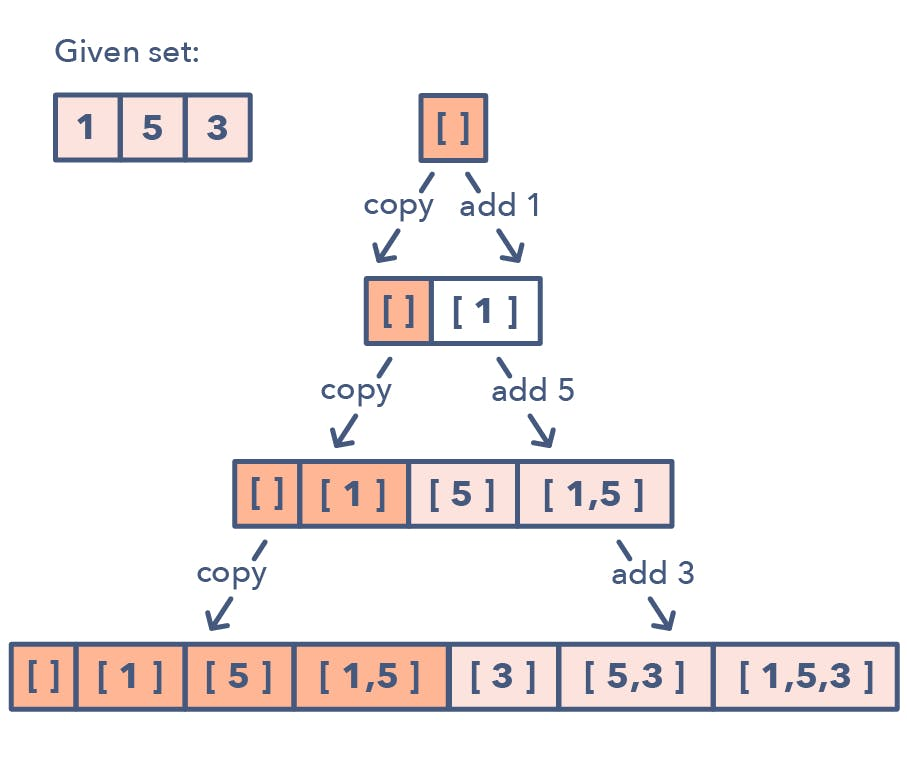
\includegraphics[width=\linewidth,keepaspectratio]{dsa7}
\end{center}		
		\end{columns}		
\end{frame}

%%%%%%%%%%%%%%%%%%%%%%%%%%%%%%%%%%%%%%%%%%%%%%%%%%%%%%%%%%%%%%%%%%%%%%
\begin{frame}[fragile]
	\frametitle{Modified binary search}
	\begin{columns}[T]
		\column{0.5\linewidth}	
Given a sorted array, linked list, or matrix, and are asked to find a certain element, the best algorithm you can use is the Binary Search.			
\begin{itemize}
			\item First, find the middle of start and end. An easy way to find the middle would be: $middle = (start + end) / 2$
			\item Or $middle = start + (end — start) / 2$
			\item If the key is equal to the number at index middle then return middle
			\item If ‘key’ isn’t equal to the index middle:
			\item Check if $key < arr[middle]$. If it is reduce your search to $end = middle — 1$
			\item Check if $key > arr[middle]$. If it is reduce your search to $end = middle + 1$
			\end{itemize}

		\column{0.5\linewidth}
			
		
\begin{center}
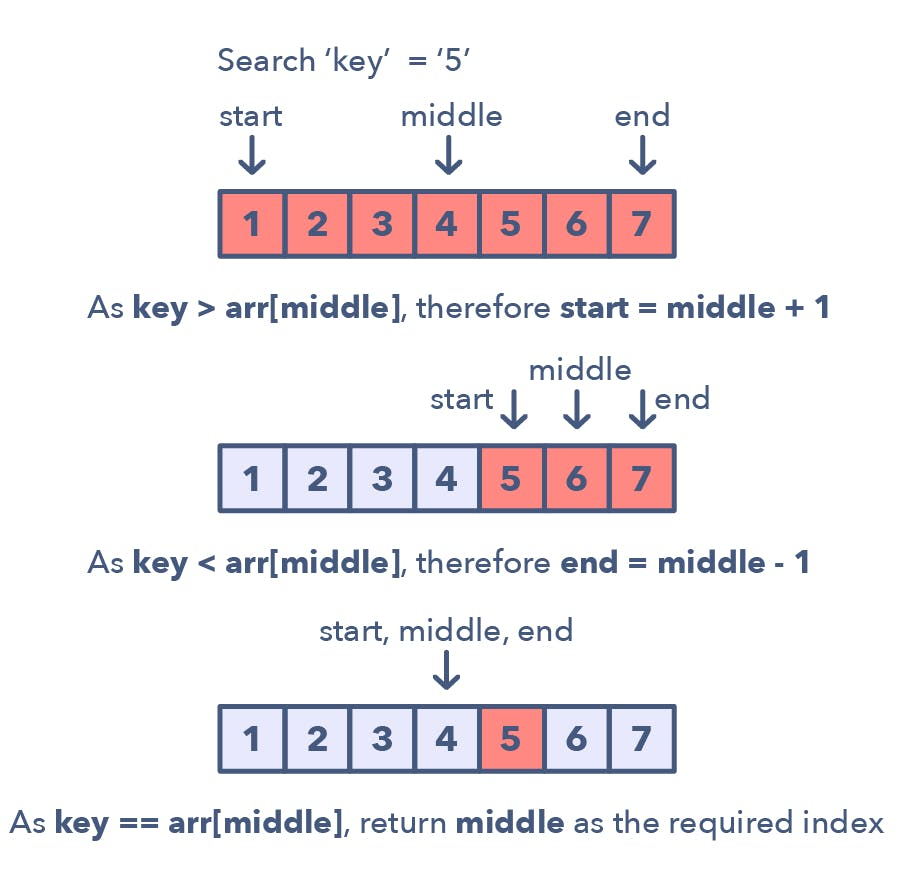
\includegraphics[width=\linewidth,keepaspectratio]{dsa8}
\end{center}		
		\end{columns}		
\end{frame}

%%%%%%%%%%%%%%%%%%%%%%%%%%%%%%%%%%%%%%%%%%%%%%%%%%%%%%%%%%%%%%%%%%%%%%
\begin{frame}[fragile]
	\frametitle{Top K elements}
	\begin{columns}[T]
		\column{0.5\linewidth}	
 	
\begin{itemize}
			\item To find the top/smallest/frequent ‘K’ elements among a given set. 			
			\item Make use of the Heap to solve multiple problems dealing with ‘K’ elements at a timeInsert ‘K’ elements into the min-heap or max-heap based on the problem.
			\item Iterate through the remaining numbers and if you find one that is larger than what you have in the heap, then remove that number and insert the larger one.
			\end{itemize}

		\column{0.5\linewidth}
			
		
\begin{center}
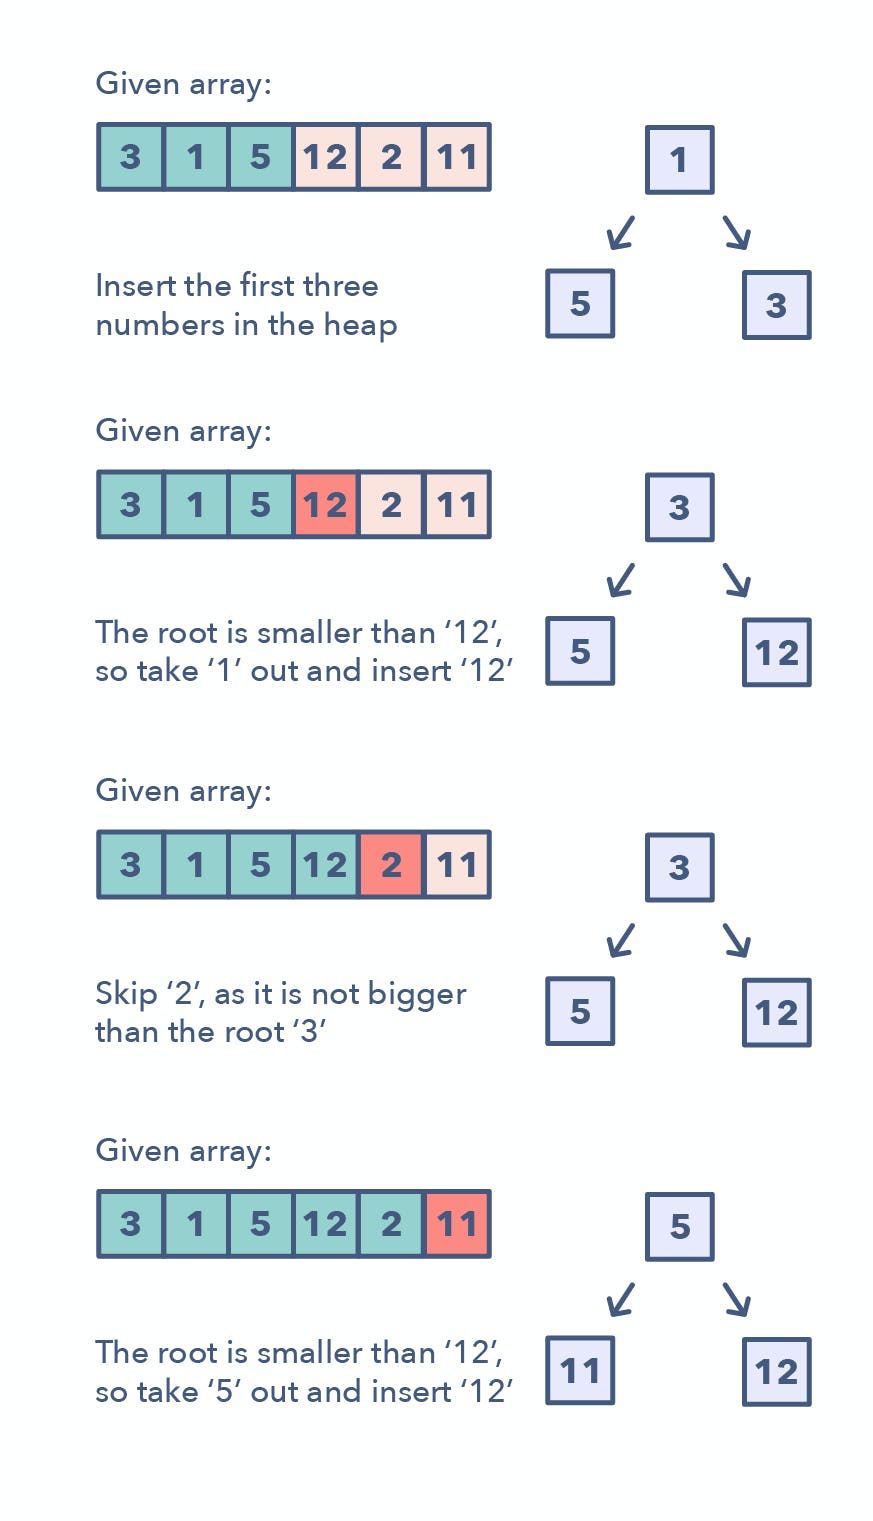
\includegraphics[width=0.8\linewidth,keepaspectratio]{dsa9}
\end{center}		
		\end{columns}		
\end{frame}



%%%%%%%%%%%%%%%%%%%%%%%%%%%%%%%%%%%%%%%%%%%%%%%%%%%%%%%%%%%%%%%%%%%%%%
\begin{frame}[fragile]
	\frametitle{K-way Merge}
	\begin{columns}[T]
		\column{0.5\linewidth}	
 	
\begin{itemize}
			\item Whenever you’re given ‘K’ sorted arrays, you can use a Heap to efficiently perform a sorted traversal of all the elements of all arrays. 			
			\item You can push the smallest element of each array in a Min Heap to get the overall minimum. 
			\item After getting the overall minimum, push the next element from the same array to the heap. 
			\item Then, repeat this process to make a sorted traversal of all elements.
			\end{itemize}

		\column{0.5\linewidth}
			
		
\begin{center}
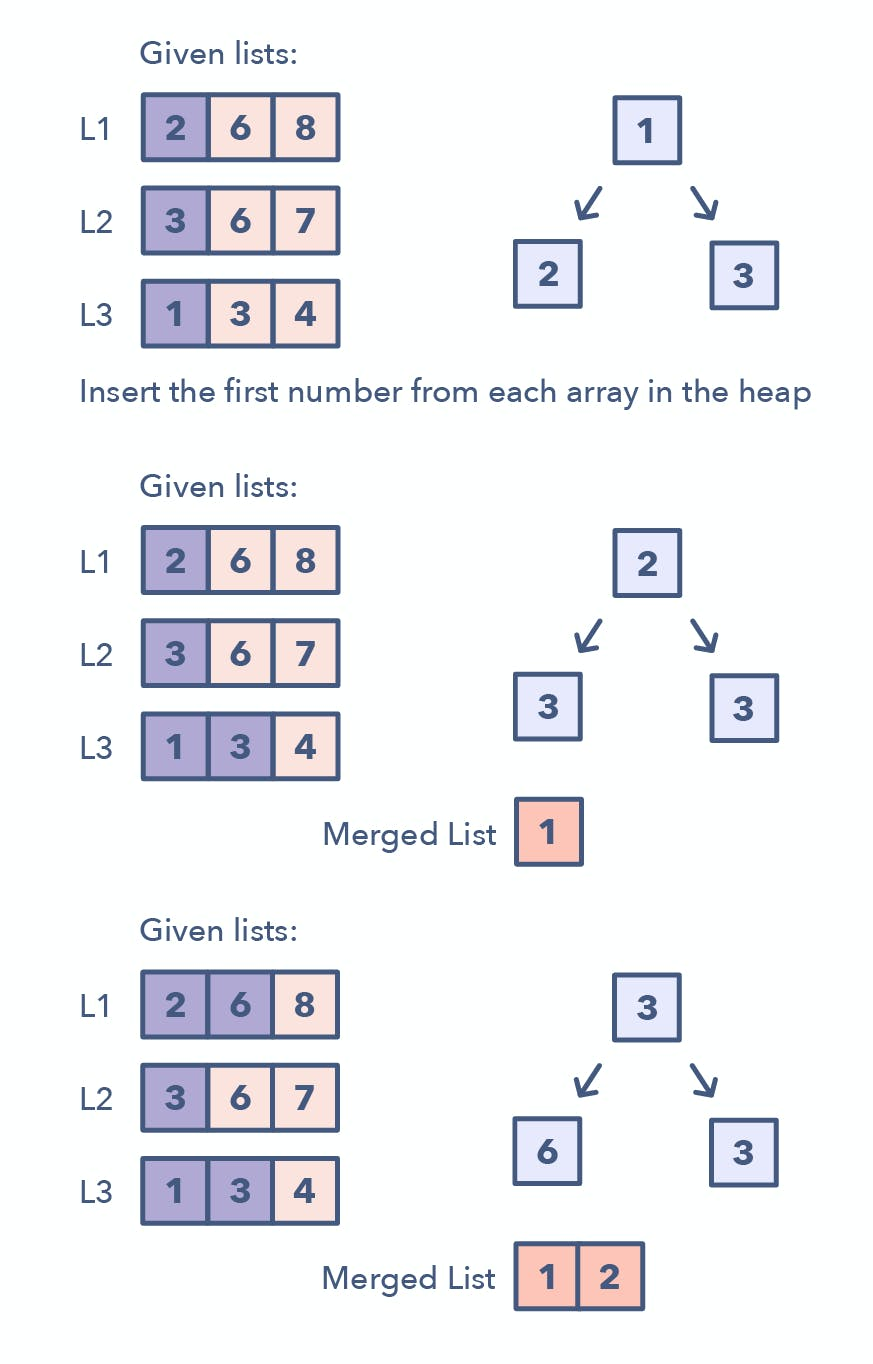
\includegraphics[width=0.8\linewidth,keepaspectratio]{dsa10}
\end{center}		
		\end{columns}		
\end{frame}



%%%%%%%%%%%%%%%%%%%%%%%%%%%%%%%%%%%%%%%%%%%%%%%%%%%%%%%%%%%%%%%%%%%%%%
\begin{frame}[fragile]
	\frametitle{Topological sort}
	\begin{columns}[T]
		\column{0.6\linewidth}	
 	To find a linear ordering of elements that have dependencies on each other.
\begin{itemize}
			\item Initialization
			\begin{itemize}
				\item Store the graph in adjacency lists by using a HashMap
				\item To find all sources, use a HashMap to keep the count of in-degreesBuild the graph and find in-degrees of all vertices
			\end{itemize}
			\item Build the graph from the input and populate the in-degrees HashMap.
			\item Find all sources: All vertices with ‘0’ in-degrees will be sources and are stored in a Queue.
			\item Sort: For each source, until the source Queue is empty:
				\begin{itemize}
					\item Add it to the sorted list.
					\item Get all its children from graph.
					\item Reduce in-degree of each child by 1.
					\item If a child’s in-degree becomes ‘0’, add it to the sources Queue.
				\end{itemize}
			\end{itemize}

		\column{0.4\linewidth}
			
		
\begin{center}
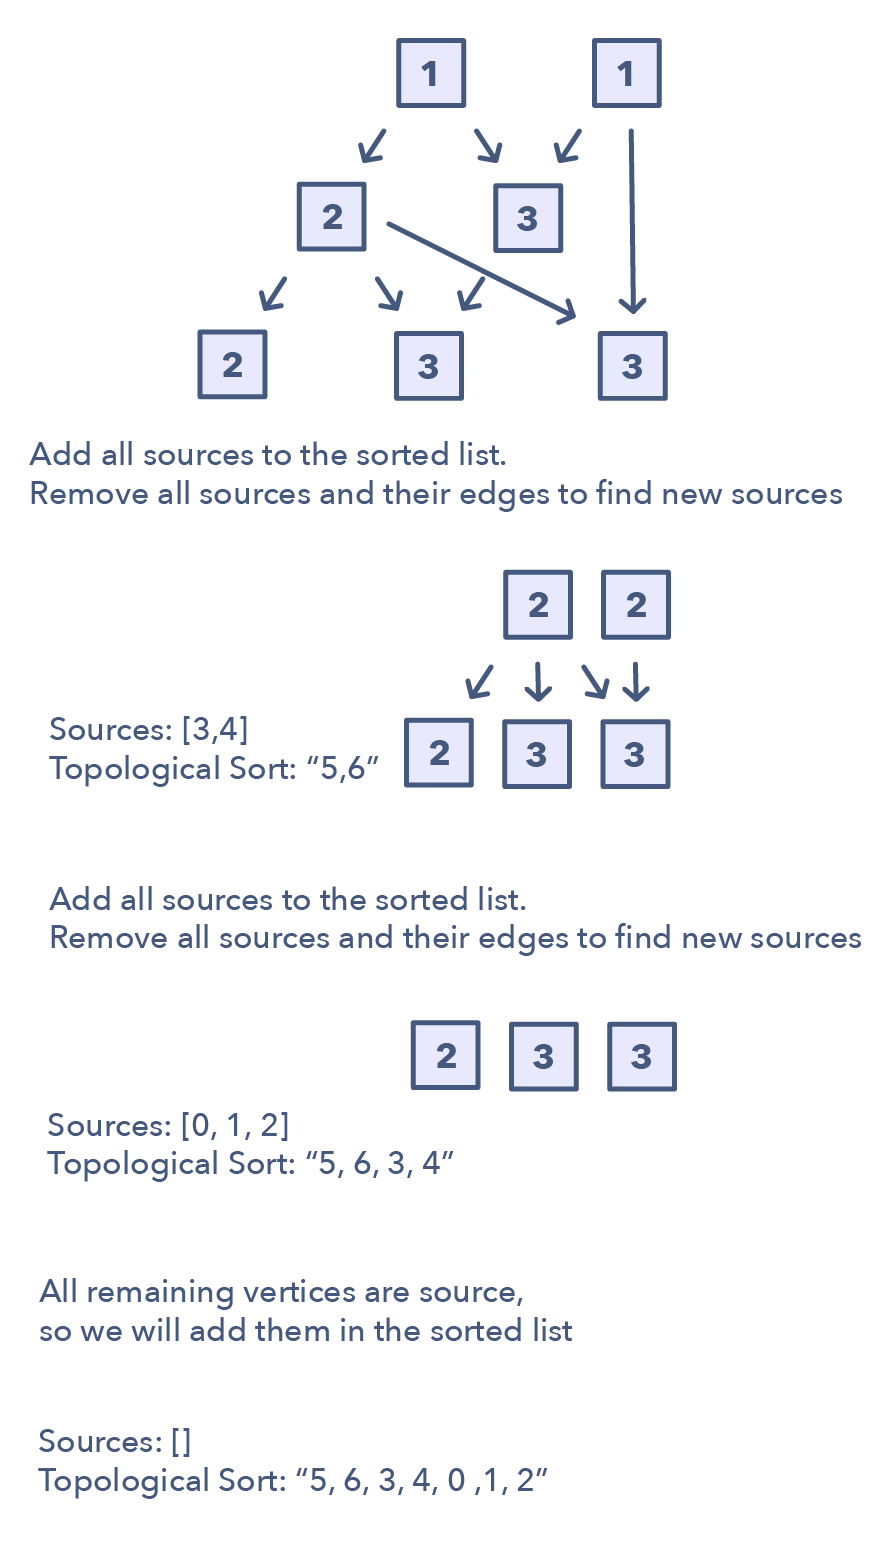
\includegraphics[width=\linewidth,keepaspectratio]{dsa11}
\end{center}		
		\end{columns}		
\end{frame}